%%%%%%%%%%%%%%%%%%%%%%%%%%%%%%%%%%%%%%%%%%%%%%%%%%%%%%%%%%%%%%%%%%%
%                                                                 %
%                            CHAPTER TWO                          %
%                                                                 %
%%%%%%%%%%%%%%%%%%%%%%%%%%%%%%%%%%%%%%%%%%%%%%%%%%%%%%%%%%%%%%%%%%%

\chapter{LITERATURE REVIEW}\label{ch:prevwork}
%\resetfootnote %this command starts footnote numbering with 1 again.

\section{Introduction}

The data versioning landscape produces a variety of different approaches and standards towards change capture.
Science agencies and organizations are only beginning to formally codify and standardize methods to capture and publish lineage information \cite{MatthewS.Mayernik201312-039}.
In comparing their methods, many systems also share the implementation of common versioning operations, suggesting an avenue for fundamental versioning properties.
While SVMs prefer to adopt th dot-decimal identifier, DOIs and other web identifiers contribute methods to connecting more expressive change documents.
Change logs are a feature which commonly appears alongside software projects and provide insight in differences between versions, but they are found very rarely among data sets.
Measuring the space between versions also appears under-explored in previous approaches.

\section{Data Versioning Operations}

Among all the systems surveyed in Section \ref{sec:system}, every one employed some form of the operations add, delete, and modify.
Literature surveys often expect versioning systems to interact with data uniformly because they are asked to perform the same functions \cite{Tagger2005}.
Different data sets, however, may utilize each of the three core operations at different rates \cite{rohtua}.
The differences help to characterize the data set in ways such as a growing set with many additions, a stable collection featuring occasional corrections, or a wildly volatile data set consisting of often deleted and replaced data files.
Understanding these would give insight into the maturity and health of a data set.

While data addition and modification remain fairly uncontroversial, there is a mild division between practical and theoretical approaches to data deletion \cite{Flouris04clotho:transparent}.
A removed object provides evidence of an erroneous activity's results or intermediary steps leading to a final product.
As a result, version management should maintain and track invalidated data instead of deleting it.
The software versioning manager GIT uses a method of compressing older data to conserve space without deleting the data \cite{Chacon:2009:PG:1618548}.
Available storage space places pragmatic constraints on the number of projects which can adopt snapshotting practices.
In applications which cannot recover erroneous data nor use it as documentation artifacts, like corrupted surveillance images.
Some high energy physics experiments cannot re-collect observational data due to cost, and as a result, they cannot replace or re-process poor quality data \cite{Cavanaugh2002}.
While the distinction between `deletion' and `invalidations' remains largely semantic, the terms' use in this document reflects an understanding of the different constraints and requirements placed on versioning systems.
As a result, invalidation is adopted as a broad, general term to also encompass data deletions.

A handful of other operations exist among version managers, but they do not prove ubiquitous across most applications.
Software versioning tools like RCS commonly feature branching and merging functions to create a versioning line separate from the stable master branch \cite{tichy1985rcs}.
Branching mostly provides an organizational role in development by allowing developers to experiment without contaminating a stable software release.
Figure \ref{GITTree} models a branching operation, showing versions C3 and C5 in branch iss53 before being merged back into the production line as C6.
Branching allows for more orderly management of versions, but does not conduct versioning itself.
Other activities provide functional operations such as locking and unlocking files from edits to prevent race conditions in branch mergers.
Locks does not introduce any new relationships but allows the tool to operate more smoothly.
Many version control tools, likewise, include functions to display the versioning tree, but this is also an ease-of-use function \cite{Dijkstra1994}.

\begin{figure}
	\centering
	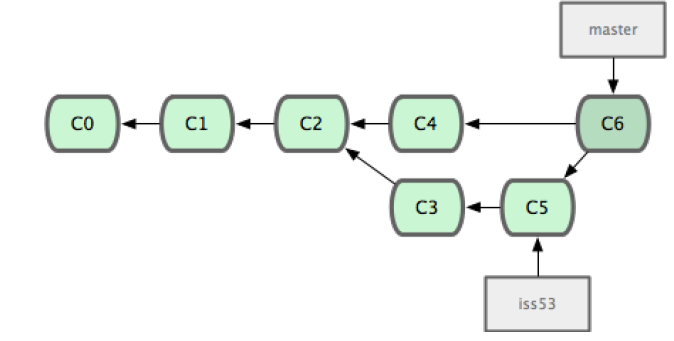
\includegraphics[scale=0.75]{figures/GITCommitTree.png}
	\caption[Example of a commit history with branching stored in GIT.]{Example of a commit history with branching stored in GIT.  Figure 3.17 from \cite{Chacon:2009:PG:1618548}}
	\label{GITTree}
\end{figure}

\subsection{Types of Change}

Another commonality across many versioning systems is differentiating between major, minor, and revision changes.
Definitions for what constitutes each category differs across applications, but the desire to do so often stems from the tradition of 3-number dot-decimal identifiers.
Barkstrom uses the ability to scientifically distinguish between two data sets as a criteria for major divisions among groupings \cite{Barkstrom2003}.
At lower levels, he notes that science teams can no longer discern scientific differences between data sets.
They observe that, instead, changes to format and structure contribute significant alterations without changing any values withing the data.
As a result, these technical changes form a second boundary to meaningfully separate minor version groupings.
Finally, the explicit values may need occasional revisions to correct lexical errors such as spelling or formatting.
Data producers will often use qualitative measures to determine the type of change occurring between versions.
Versioning system users wish to achieve insight into the type of change that occurs between versions.

The exact category that a particular change falls into can be controversial.
The decision to provide concentration units from parts per million to milligrams per milliliter poses a Technical change for a data producer.
However, for a data consumer, the alteration may be viewed as a Scientific change as it invalidates the methods they had previously used.
The conflict in view illustrates the data consumer-producer dynamic.
In general, data producers control the versioning methods, but data consumers determine a change's impact through use.
Producers tend to use versioning systems to ensure data quality of service through audits and recovery tools \cite{Cavanaugh2002}.
Meanwhile, a consumer will analyze the historical changes and determine the impact this may have on their data use.
As a result, this means that data versioning systems must communicate a dynamic view of the changes in a system contextualized by the user of that data.

Version managers often disagree at the point many technical changes sufficiently modifies a data set that it comprises a scientific change.
As determining changes in science requires expert understanding over a domain, different measures should be explored to address the distinction.

\section{Identifiers}

The most widely identifier scheme associated with versioning is the dot-decimal identifier \cite{Stuckenholz:2005:CEV:1039174.1039197}.
Whenever, a new version is made, it receives an identifier with one of the numbers incremented as seen in Figure \ref{RCSTree}.
Such a procedure fails to communicate the extent of a change because, regardless of the amount, the identifier will increment only one number.
Changes to the left-most number often signify a more important change.
Many software applications use the 3-number Major.minor.revision format in labeling software releases.
Numbering the version this way, however, does allow computers and readers to quickly parse the version name and discern that a change has occurred, but not much value exists beyond that \cite{Dijkstra1994}.
Most importantly, it groups together changes from the lower spectrum of minor or major change with those in the upper, more impactful, changes.
Obtaining a clear characterization of a version change is difficult without a longer series of numbers.
In addition, version numbers capture the overall change of a data set, but users may not interact with collections that way, only caring about parts of the data or certain kinds of change.
There is also little standardization or formal requirements in naming methods.
Ubuntu utilizes a dot-decimal version labeling scheme where the two number identifier corresponds to the year-month values of the release \cite{Ubuntu}.
A common method used to address the distinction between versions is a human-readable change log, further discussed in Section \ref{sec:changelog}.

The discourse on DOIs highlights the importance of understanding the limitations of particular identifier schemes.
With respect to Figure \ref{table:Duerr}, no identification scheme fits the description of a scientific identifier.
Duerr, et al., define a use case to make the argument that scientifically unique identifiers are necessary, ``to be able to tell that two data instances contain the same information even if the formats are different" \cite{Duerr2011}.
A possibility to consider is that identifiers may require incorporation into a data model to discern between scientific differences.
An identifier works well in revealing the characteristics of an individual object, but it should not be expected to explain its relationship with other objects.
A data model provides better insight into the different roles objects play in a relationship.
DOIs also provide a new means to identify versions using URIs which can be dereferenced to provide change information or the data depending on the context.

Using identifiers to convey extended versioning information becomes more difficult with the adoption of distributed version managers like GIT \cite{cederqvist2002version}.
Each participant in the federated repository is the master of their personal copy of the code.
Upon completion of their distribution's part, they may request that it be pulled into another participant's distribution.
While each developer's individual repository can follow a linear identifier scheme, the identifiers would not work as the overall project bounces around different primary repositories with mismatching sequential identifiers.
The dot-decimal identifier scheme could be made to work in such an environment by severely limiting the distributed manager's utilized features.
Figure \ref{fig:federated} illustrates a workflow which utilizes distributed repositories to manage very active public software projects.
Each lieutenant developer manages a section of the overall code, and they dampen the number of requests made to the dictator by collecting changes and submitting them over longer intervals.
As a result, relying on identifiers to convey and contain versioning information limits the evolution of new and valuable methods of processing change in digital objects.

\begin{figure}
	\centering
	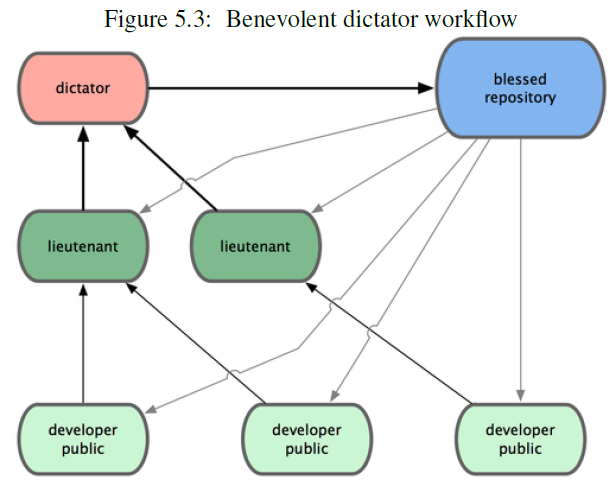
\includegraphics[scale=0.85]{figures/federatedGit.png}
	\caption[A distributed workflow to control for volatile versioning behavior.]{A distributed workflow to control for volatile versioning behavior.  From  \cite{cederqvist2002version}.}
	\label{fig:federated}
\end{figure}

\section{Change Logs} \label{sec:changelog}

Change logs, artifacts resulting from the versioning process, play a major role filling in gaps between versions.
The logs document changes and explain, in human language, motivations behind the modifications \cite{uel1037}.
Since identifiers denote that a change has occurred, the logs provide details on how the changes modify an object's attributes.
They demonstrate a need and utility in understanding the deeper content of change beyond knowing that an object did transform.
While some data sets will provide a change log, software projects have normalized their use in version release documentation.
As a result, these projects provide a basis for understanding the value these logs can supply data sets with multiple versions.
The change log's common drawback is the limitation to only human readable text.
Wider adoption among data sets may be possible by making these texts machine computable.

Open source projects use change logs more consistently than data projects, which usually sport only use documentation.
Logs play an important communication role in these projects since developers can contribute without having been part of the original development team.
The change logs allow developers to link bugs and errors with their corrections in new versions of the code \cite{Chen:2004:OCL:990374.990391}.
The links gives insight into motivations behind particular design decisions.
Logs linked with version releases also provide feedback to the user community that corrections have been addressed, in addition to ensuring that improvements drive modifications to the code base.
An identifier cannot communicate these qualities while remaining succinct.
Some research has been done to determine the health of a development project based on the number and length of change logs released over time \cite{German03automatingthe}.
Little work has been done to make change logs machine-computable, as many of these documents remain in human-readable text only.
Research done involving change log content must manually link entries with computable meta-data such as the introduction of new features with the emergence of new bugs \cite{6132954}.
While machines may still be significantly removed from the ability to comprehend the impact of changes made to a data set or software code, they are currently opaquely blocked from consuming any of the content within logs more than understanding they contain text.
The transition between different versions of large data sets is then left largely up to the human user's ability to understand and process the modifications mentioned within the change log.

\subsection{Structured Data}

The Resource Description Framework in Attributes (RDFa) framework encodes linked data vocabularies into HTML documents, and provides an opportunity to make change logs machine interpretable. \cite{Adida2015}.
\begin{figure}
	\centering
	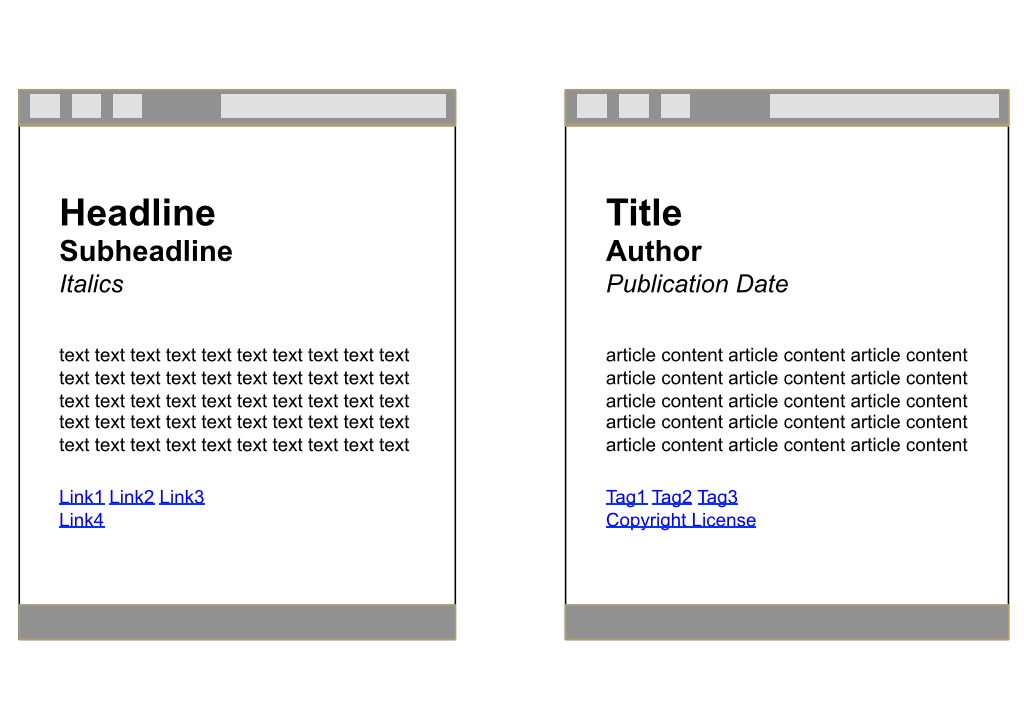
\includegraphics[scale=0.40]{figures/RDFaSemantics.png}
	\caption[Illustration of the difference in what autonomous systems see when crawling a web page and what humans see when reading the same material.]{Illustration of the difference in what autonomous systems see when crawling a web page and what humans see when reading the same material. Figure 1 from \cite{Herman2015}}
	\label{RDFa}
\end{figure}Figure \ref{RDFa} illustrates the semantic difference between what web crawlers and what humans see when they consume web pages.
People intuitively understand that certain strings represent meaningful information based on location and style.
RDFa seeks to encode that understanding natively for effective machine consumption.
Extending this approach into publishing change logs, will allow linked data to capture the metaphorical meat of change content.

The implementation requires changing publishing practices from plain-text documents to something structured-data compatible such as HTML.
The change also has the added benefit of making the logs available on-line, and thus, more openly accessible to data users through the utilization of web based search engines.
Large companies such as Google have already begun equipping their web crawlers to consume structured data such as RDFa from web pages.
RDFa has already had significant success in adoption across a variety of web publication platforms and eases the search for their content \cite{Bizer2013}.
The design of RDFa focuses on describing the web page's content through markup \cite{Herman2015}.
The underlying or resulting versioning data model may not conform with the format of content presented in the change log.
Poor affinity would lead to a poorly structured graph or missing content, undermining the value gained by encoding linked data into the change log.
As a result, another method using JavaScript Object Notation for Linked Data (JSON-LD) was pursued since its purpose is to store data separate from visible content.

The JSON data format allows web pages to store data for JavaScript applications within the document.
It utilizes a simple and robust syntax to accommodate a wide variety of content.
JSON-LD extends the original specification by defining rules which allow entries to resolve as web vocabularies, giving them a meaningful context \cite{JSONLD}.
Because it stores data separate from visible content, JSON-LD does not need to adhere with the constraints of visible content.
Every linked data triple must instead be explicitly defined, meaning that resulting documents may likely be much larger than their RDFa counterparts.

\section{Change Distance}

A major function of versions is to communicate the amount of change which exists between two versions.
The quantity plays a major role in determining the freshness of data within a collection, indicating its pertinence to new projects \cite{Bouzeghoub:2004:FAD:1012453.1012464}.
Additionally, changing versions are often used to signal other applications downstream that a new version may be necessary to adopt data improvements \cite{TILMES2011548}.
Many efforts currently to compute a distance measure relies on data provenance.
Formalizing operations on provenance remains an active field of research \cite{Ainy:2015:ASD:2806416.2806429}.
Other approaches relate to determining semantic similarity in trying to summarize the data set and computing a distance measure \cite{Hliaoutakis06informationretrieval}.

\subsection{Provenance Distance}

Previous endeavors to extract insight into data set performance or behavior have provided exciting results \cite{dai2014provenance}.
The research, however, generally studies the current state of an object's provenance rather than compare two provenance graphs.
As stated previously, versions result from slight variations between the provenance of two objects.
The connection suggests that studying the variations' magnitudes will help predict the change's impact.
The measurement known as provenance distance seeks to determine the impact of changes in provenance on new data versions through measuring graph edit distances.

\begin{figure}
	\centering
	\begin{adjustbox}{addcode={\begin{minipage}{\width}}{
					\caption[Provenance graph of a Level 3 data product, showing the inter-relations between different data products in generating the final product.]{Provenance graph of a Level 3 data product, showing the inter-relations between different data products in generating the final product.  Figure 2 from \cite{TILMES2011548}}\end{minipage}},rotate=90,center}
		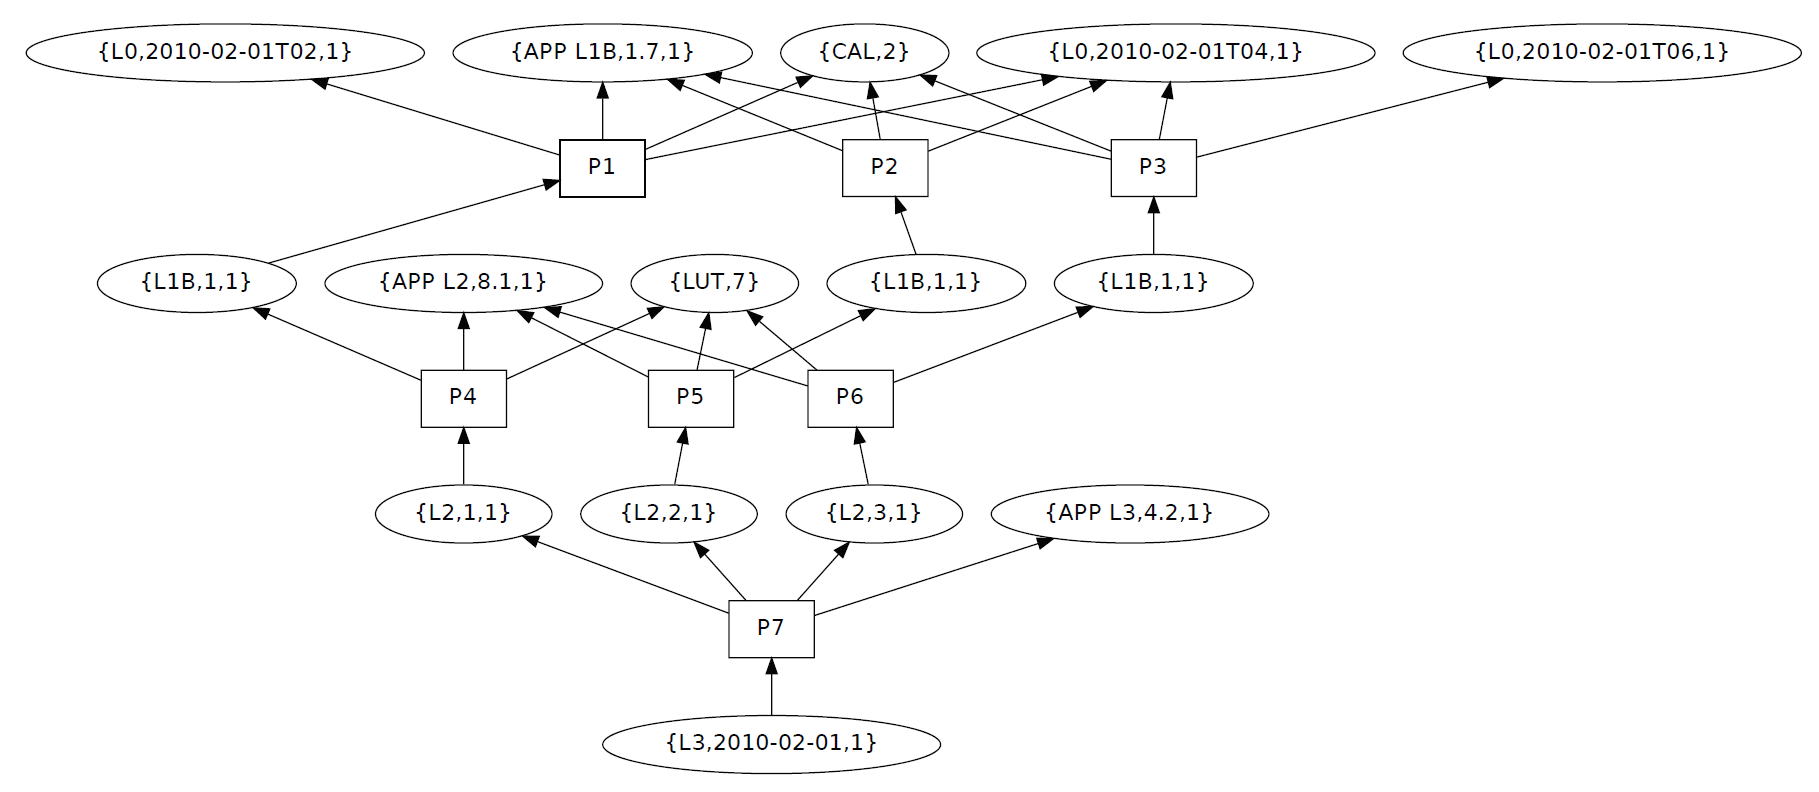
\includegraphics[scale=0.5]{figures/OzoneProvGraph.png}
	\end{adjustbox}
	\label{ProvGraph}
\end{figure}

The first ingredient necessary to calculate provenance distance is a linked data graph capturing the sequence of events leading to the old and new objects' creation, like the one shown in Figure \ref{ProvGraph}.
The graph shows the multiple lower level products involved in creating a Level 3 ozone indicator.
This can be accomplished through the use of previously mentioned provenance models, but these graphs are not widely available.
Using PROV to represent provenance data in a semantic model produces an acyclic directed graph with labeled nodes.
As a result, the provenance distance problem reduces to similarity measurement.
When calculating the similarity measurement of two graphs, algorithms determine how far the graphs are from being isomorphic \cite{Cao2013}.
Node labeling simplifies the similarity measurement process by providing nodes which must match together, and greatly reduces the complexity from computing generalized graphs.
Graph Edit Distance, counting the edits necessary to transform one graph into another, provides a quantitative measure to associate with this process  \cite{Gao2010}.
Some variations count edge changes \cite{Goddard:1996:DGU:246962.246972}.

In Figure \ref{GraphEdit}, the left graph transforms through a move of edge 1 and a rotation of edge 4, resulting in an edit distance of two.
Such changes in a provenance graph would demonstrate an alteration in dependencies between objects used to generate a final notable product.
Isolating changes responsible for differences in provenance can become difficult in complex environments as Tilmes observes in 2011, 
\begin{quotation}
	Consider the relatively common case of the calibration table, which is an input to the L1B process, changing. Even though the version of the L2 or L3 software hasn't changed, the data files in the whole process have been affected by the change in the calibration.
\end{quotation} \cite{TILMES2011548}.
L-number is shorthand for the level system featured in Figure \ref{NASALevels}.
While provenance distance may be straight-forward to calculate, the indicator hides many insights into an object's behavior.

\begin{figure}
	\centering
	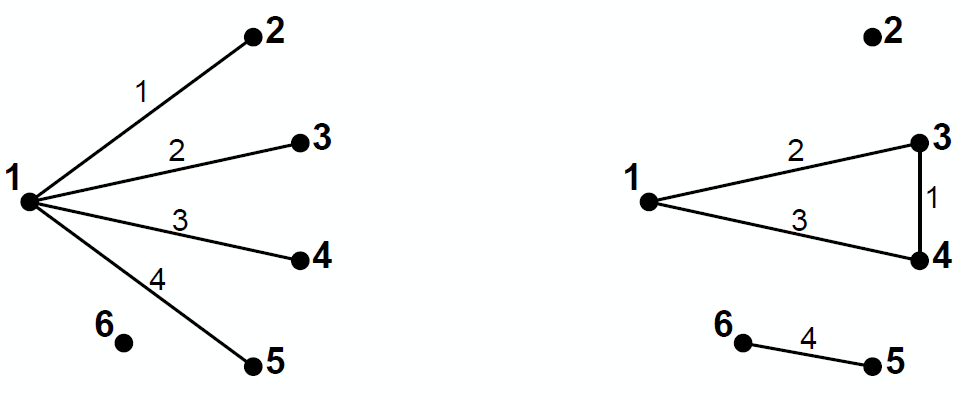
\includegraphics[scale=0.40]{figures/GraphEdit.png}
	\caption[The labeled graph on the left transforms into the right graph under two edge edits.]{The labeled graph on the left transforms into the right graph under two edge edits. Figure 2 from \cite{Goddard:1996:DGU:246962.246972}}
	\label{GraphEdit}
\end{figure}

Methods to provide quality of service boundaries leveraging provenance already exist which compare workflows based on performance criteria \cite{2015:CAA:2778374.2778504}.
These procedures focus primarily on quick retrieval and efficient storage instead of capitalizing on the latent information accessed by reasoning across data set versions \cite{tan2004research}.
Using only provenance data is insufficient to give insight into a change's impact because it does not provide information on structural or content differences which is what change logs provide.
Measuring a change's impact with accuracy comparable to a change log requires a more detailed understanding and description than provenance can provide  \cite{Bose:2005:LRS:1057977.1057978}.
Sufficiently precise versioning measurements cannot be provided by provenance distance, but it could indicate the confidence of versioning results, which is out of scope for this project.

\section{Summary}

In order to better formalize data versioning information, an approach must be developed leveraging common aspects of very disparate versioning systems.
A data model based around versioning operations instead of impact remains largely untouched across the field.
Version identifiers must additionally be untangled from communicating change distance which change logs accomplish with greater detail.
The logs, in turn, need to be extended for machines to consume, easing adoption as data set size grows through automation.
Change measures utilizing version graphs rather than provenance graphs are also under-explored.
Chapter \ref{ch:model} presents a model to create a versioning graph.

%%% Local Variables:
%%% mode: latex
%%% TeX-master: t
%%% End:
